% Options for packages loaded elsewhere
\PassOptionsToPackage{unicode}{hyperref}
\PassOptionsToPackage{hyphens}{url}
%
\documentclass[
  11pt,
]{article}
\usepackage{lmodern}
\usepackage{amssymb,amsmath}
\usepackage{ifxetex,ifluatex}
\ifnum 0\ifxetex 1\fi\ifluatex 1\fi=0 % if pdftex
  \usepackage[T1]{fontenc}
  \usepackage[utf8]{inputenc}
  \usepackage{textcomp} % provide euro and other symbols
\else % if luatex or xetex
  \usepackage{unicode-math}
  \defaultfontfeatures{Scale=MatchLowercase}
  \defaultfontfeatures[\rmfamily]{Ligatures=TeX,Scale=1}
  \setmainfont[]{Arial}
\fi
% Use upquote if available, for straight quotes in verbatim environments
\IfFileExists{upquote.sty}{\usepackage{upquote}}{}
\IfFileExists{microtype.sty}{% use microtype if available
  \usepackage[]{microtype}
  \UseMicrotypeSet[protrusion]{basicmath} % disable protrusion for tt fonts
}{}
\makeatletter
\@ifundefined{KOMAClassName}{% if non-KOMA class
  \IfFileExists{parskip.sty}{%
    \usepackage{parskip}
  }{% else
    \setlength{\parindent}{0pt}
    \setlength{\parskip}{6pt plus 2pt minus 1pt}}
}{% if KOMA class
  \KOMAoptions{parskip=half}}
\makeatother
\usepackage{xcolor}
\IfFileExists{xurl.sty}{\usepackage{xurl}}{} % add URL line breaks if available
\IfFileExists{bookmark.sty}{\usepackage{bookmark}}{\usepackage{hyperref}}
\hypersetup{
  pdftitle={Effects of Advanced Trauma Life Support® Training Compared to Standard Care on Adult Trauma Patient Outcomes: Initiating A Cluster Randomised Trial},
  hidelinks,
  pdfcreator={LaTeX via pandoc}}
\urlstyle{same} % disable monospaced font for URLs
\usepackage[margin=2.5cm]{geometry}
\usepackage{longtable,booktabs}
% Correct order of tables after \paragraph or \subparagraph
\usepackage{etoolbox}
\makeatletter
\patchcmd\longtable{\par}{\if@noskipsec\mbox{}\fi\par}{}{}
\makeatother
% Allow footnotes in longtable head/foot
\IfFileExists{footnotehyper.sty}{\usepackage{footnotehyper}}{\usepackage{footnote}}
\makesavenoteenv{longtable}
\usepackage{graphicx}
\makeatletter
\def\maxwidth{\ifdim\Gin@nat@width>\linewidth\linewidth\else\Gin@nat@width\fi}
\def\maxheight{\ifdim\Gin@nat@height>\textheight\textheight\else\Gin@nat@height\fi}
\makeatother
% Scale images if necessary, so that they will not overflow the page
% margins by default, and it is still possible to overwrite the defaults
% using explicit options in \includegraphics[width, height, ...]{}
\setkeys{Gin}{width=\maxwidth,height=\maxheight,keepaspectratio}
% Set default figure placement to htbp
\makeatletter
\def\fps@figure{htbp}
\makeatother
\setlength{\emergencystretch}{3em} % prevent overfull lines
\providecommand{\tightlist}{%
  \setlength{\itemsep}{0pt}\setlength{\parskip}{0pt}}
\setcounter{secnumdepth}{5}
\usepackage{float}
\newfloat{textbox}{thp}{}
\usepackage{setspace}
\usepackage[font={small}]{caption, subfig}
\usepackage{titlesec}
\usepackage{multicol}
\usepackage{mdframed}
\usepackage{fancyhdr}
\newcommand{\bcenter}{\begin{center}}
		\newcommand{\ecenter}{\end{center}}
\renewcommand{\topfraction}{.85}
\renewcommand{\bottomfraction}{.7}
\renewcommand{\textfraction}{.15}
\renewcommand{\floatpagefraction}{.66}
\renewcommand{\baselinestretch}{1.0}
\titleformat{\section}{\normalfont\fontsize{11}{14}\bfseries}{\thesection}{1em}{}
\titleformat{\subsection}{\normalfont\fontsize{11}{14}\bfseries}{\thesubsection}{1em}{}
\titleformat{\subsubsection}{\normalfont\fontsize{11}{14}\bfseries}{\thesubsubsection}{1em}{}
\titlespacing{\section}{0em}{0.5em}{0.25em}
\titlespacing{\subsection}{0em}{0.5em}{0.25em}
\titlespacing{\subsubsection}{0em}{0.5em}{0.25em}
\setlength{\parskip}{0.25em}
\setlength{\abovecaptionskip}{0.25em}
\setlength{\belowcaptionskip}{0.25em}
\setlength{\floatsep}{0.25em}
\setlength{\textfloatsep}{0.5em}
\setcounter{topnumber}{1}
\setcounter{bottomnumber}{1}
\setcounter{totalnumber}{2}
\fancyhead[CO,CE]{ATLS® vs Standard Care in Adult Trauma Patients}
\fancyhead[LO,LE]{}
\fancyhead[RO,RE]{}
\newlength{\cslhangindent}
\setlength{\cslhangindent}{1.5em}
\newenvironment{cslreferences}%
  {}%
  {\par}

\title{Effects of Advanced Trauma Life Support\textsuperscript{®} Training Compared to Standard Care on Adult Trauma Patient Outcomes: Initiating A Cluster Randomised Trial}
\author{}
\date{\vspace{-2.5em}}

\begin{document}
\maketitle

\pagestyle{fancy}

\hypertarget{summary-and-objectives}{%
\section{Summary and Objectives}\label{summary-and-objectives}}

Trauma is a global health issue.\textsuperscript{\protect\hyperlink{ref-injuries2020}{1},\protect\hyperlink{ref-GBD2020}{2}} Many training programmes have been developed to help physicians in the early care of trauma patients, but high quality evidence on the effects of implementing these programmes on patient outcomes is missing.\textsuperscript{\protect\hyperlink{ref-Mohammad2013}{3}--\protect\hyperlink{ref-Jin2021}{6}} With the support of the Laerdal Foundation and the Swedish Research Council we conducted a pilot and feasibility study in India comparing the effects of the two most widely used trauma life support training programmes, the Advanced Trauma Life Support\textsuperscript{®} (ATLS\textsuperscript{®}) and the Primary Trauma Care (PTC) programmes, on patient outcomes.\textsuperscript{\protect\hyperlink{ref-GerdinWuxe4rnberg2022}{7}} This pilot showed that a full scale trial is feasible, but that the full scale trial should focus on ATLS\textsuperscript{®} using a stepped wedge design and include a careful local adaption of how ATLS\textsuperscript{®} is implemented. We have now planned this full scale trial and here we apply for funding for 18 months with the objectives to:

\begin{enumerate}
\def\labelenumi{\arabic{enumi}.}
\tightlist
\item
  finalise local adaptation, implementation and data collection methods; and
\item
  initiate the full scale trial in two hospitals.
\end{enumerate}

\hypertarget{background-information}{%
\section{Background Information}\label{background-information}}

Each year, 4.3 million people die from trauma.\textsuperscript{\protect\hyperlink{ref-injuries2020}{1}} In the age group 10-49 years trauma is the largest cause of disability adjusted life years.\textsuperscript{\protect\hyperlink{ref-GBD2020}{2}} Most preventable trauma deaths are caused by clinical judgement errors during early care including airway management and haemorrhage control.\textsuperscript{\protect\hyperlink{ref-Roy2017}{8}} The Advanced Trauma Life Support\textsuperscript{®} (ATLS\textsuperscript{®}) is the most established trauma life support training programme aiming to improve early hospital trauma care, and more than one million physicians in over 80 countries have been trained in ATLS\textsuperscript{®} since the first course in 1978.\textsuperscript{\protect\hyperlink{ref-acsAtls2018}{9}} Uptake in low- and middle income countries (LMIC) has been slow, potentially due to high costs.\textsuperscript{\protect\hyperlink{ref-Kadhum2020}{5}} Three randomised controlled studies show that ATLS® improves knowledge and clinical skills,\textsuperscript{\protect\hyperlink{ref-Mohammad2013}{3}} but there are no randomised controlled trials or high-quality quasi-experimental trials indicating that ATLS\textsuperscript{®} or similar programmes improve patient outcomes.\textsuperscript{\protect\hyperlink{ref-Mohammad2013}{3}--\protect\hyperlink{ref-Jin2021}{6}} We conducted an updated systematic review (Text box 1) and estimated a pooled risk ratio of 0.82 (95\% CI 0.60; 1.11) from ten heterogeneous (I\textsuperscript{2} 0.91) observational studies on the effect of ATLS on mortality (Figure \ref{fig:forest-plot}), indicating that ATLS® training may have an effect on mortality, but that the quality of evidence is poor.

\begin{textbox}
\begin{mdframed}[frametitle={Text box 1: Systematic Review}, nobreak=true, backgroundcolor=blue!10]
We performed a systematic literature search in the Medline, Embase, Cochrane, Web of Science, CINAHL and Google Scholar databases (PROSPERO ID CRD42022373977). The last search was conducted on November 11, 2022. We developed the search strategy in Medline (Ovid) in collaboration with librarians at the Karolinska Institutet University Library. We limited the search to English language articles, searched all databases from inception, and screened a total of 7896 records. We used a random effects model to pool estimates across studies.
\end{mdframed}
\end{textbox}

\begin{figure}
\centering
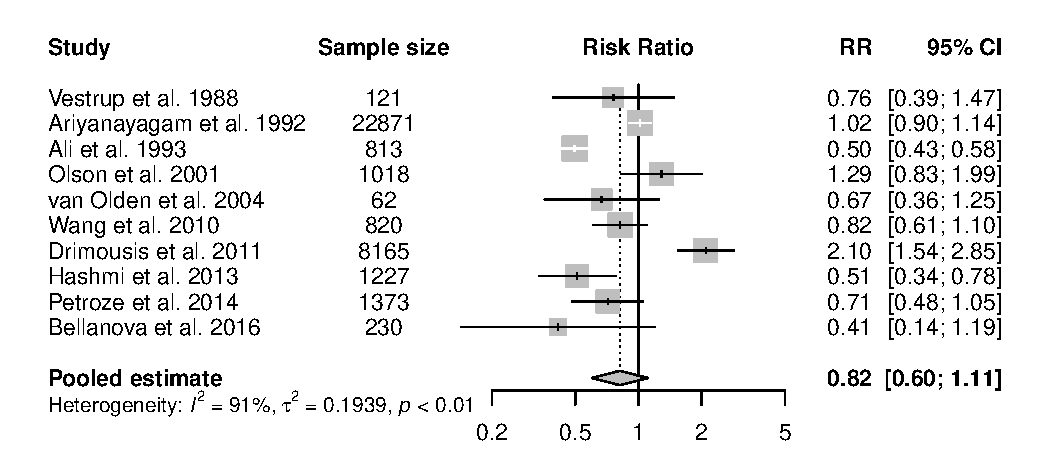
\includegraphics{forest-plot.pdf}
\caption{\label{fig:forest-plot}Systematic review on the effect of Advanced Trauma Life Support\textsuperscript{®} training on in-hospital mortality. A Risk Ratio (RR) less than 1 indicates that ATLS\textsuperscript{®} training reduces in-hospital mortality. Abbreviations: CI Confidence Interval.}
\end{figure}

\hypertarget{clinical-significance-of-preliminary-studies}{%
\section{Clinical Significance of Preliminary Studies}\label{clinical-significance-of-preliminary-studies}}

This application was developed jointly by the parties participating in the Trauma life support training Effectiveness Research Network (\href{https://www.tern.network}{tern.network}). We have conducted multicentre trauma research in India since 2013 (\href{https://www.titco.org}{titco.org}), including the pilot study (ClinicalTrials.gov NCT05417243) between April 2022 and February 2023, for which we published the protocol.\textsuperscript{\protect\hyperlink{ref-GerdinWuxe4rnberg2022}{7}} Since 2013, we have collected data from 35,970 patients across 13 hospitals, out of which 13,979 patients fit the eligibility criteria of this trial. Among eligible patients the average in-hospital mortality is 25\%. Our pilot study enrolled 375 patients from seven hospitals across India (unpublished data) and shows that it is feasible to conduct the proposed trial with a high recruitment rate (78\%), low loss to follow-up rate (1\%), and low missingness in key variables (mean 1\%). We conducted 19 semi-structured interviews with trauma patients, caregivers, and community representatives (unpublished data) to involve patients in the planning of this trial and to understand which outcomes they perceive as important. The interviews showed high acceptability of our research and emphasised the importance of better recovery before discharge and functional outcomes at and after discharge, including pain, mobility and self-care activities. The interviews also highlighted return to work as an important outcome.

\hypertarget{experimental-design}{%
\section{Experimental Design}\label{experimental-design}}

We plan to conduct a batched stepped-wedge cluster randomised controlled trial comparing the effects of ATLS\textsuperscript{®} with standard care. Based on our pilot study, we decided to compare only ATLS\textsuperscript{®} with standard care because including both ATLS\textsuperscript{®} and PTC in a three-armed trial would require a substantially larger number of clusters and in choosing between ATLS\textsuperscript{®} and PTC, ATLS\textsuperscript{®} is the most established and widely available programme. Our pilot also showed that the costs associated with training physicians in ATLS\textsuperscript{®} and PTC were the same. In this application, we apply for funding to initiate the trial in two hospitals so that we can finalise local adaptation, implementation and data collection methods, but we describe the full scale trial below.

\hypertarget{trial-design}{%
\subsection{Trial design}\label{trial-design}}

We report our research plan according to the Consolidated Standards Of Reporting Trials (CONSORT) extension for stepped-wedge cluster randomised controlled trials.\textsuperscript{\protect\hyperlink{ref-Hemming2018}{10}} The trial will be registered with the Clinical Trials Registry of India and ClinicalTrials.gov. The stepped-wedge trial is a uni-directional cross-over trial but the time point when clusters cross-over from standard care to the intervention is randomised.\textsuperscript{\protect\hyperlink{ref-Hemming2015}{11}} Each cluster will be a tertiary hospital in India. We will conduct this trial in India because of 1) our established collaboration with Indian institutions and experience in conducting multicentre studies in this setting, and 2) physicians in India are not routinely trained in ATLS® or similar programmes. In the full scale trial, we plan to roll out ATLS\textsuperscript{®} to 30 clusters over six batches, so there will be five clusters in each batch (see Figure \ref{fig:trial-design}). The clusters in each batch will be randomised to one of five implementation sequences, with one clusters randomised to each implementation sequence. All clusters will transition through three phases:

\begin{enumerate}
\def\labelenumi{\arabic{enumi}.}
\tightlist
\item
  \textbf{Standard care phase (minimum four months)}, during which we will collect baseline data and locally adapt the implementation of ATLS\textsuperscript{®}
\item
  \textbf{Transition phase (one month)}, during which the training is delivered
\item
  \textbf{Intervention phase (minimum four months)}, during which the effects of training are measured
\end{enumerate}

The total duration of these three phases will be 13 months. The implementation sequence determines how long the phases of standard care and intervention are.

\hypertarget{design-justification}{%
\subsection{Design justification}\label{design-justification}}

We use the cluster randomised design because the intervention cannot be randomised at the individual patient level. We use the stepped-wedge design for two reasons. First, this design is statistically more efficient than the parallel cluster design when the number of clusters is limited. Second, the stepped-wedge design is likely to enhance participation and engagement because all clusters receive the intervention. The batched stepped-wedge design further improves feasibility as it does not require all clusters to start at the same time, and it is robust to potential delays in cluster recruitment.\textsuperscript{\protect\hyperlink{ref-Kasza2022}{12}}

\begin{figure}
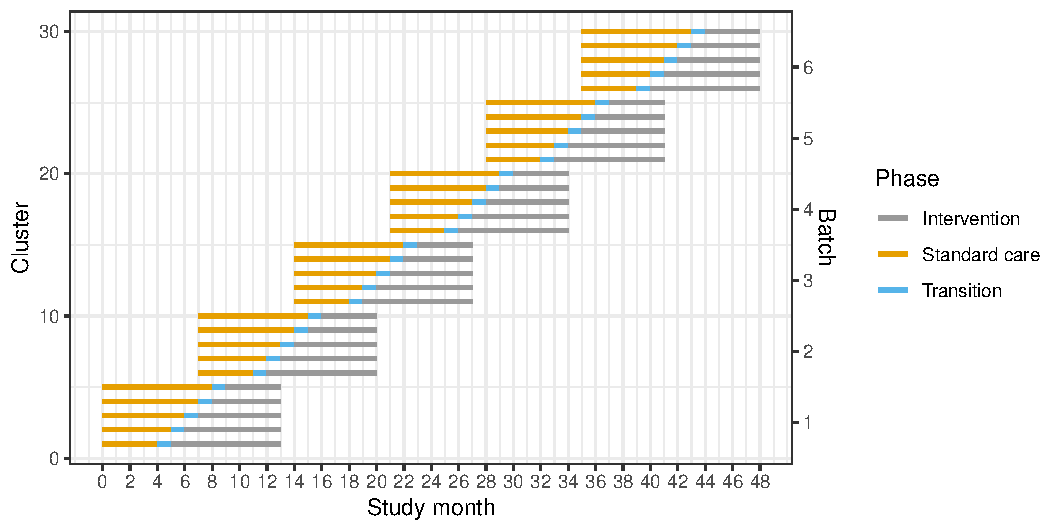
\includegraphics{trial-design-figure-30-clusters-5-sequences-6-batches-6-batches-overlap-4-min-standard-care-4-min-intervention-1-transition-months-0-transition-overlap} \caption{Trial design. Lines represent the duration of patient enrolment across clusters and phases. Clusters will be sequentially allocated to a batch based on when they enter the study. Within each batch clusters will then be randomised to an intervention implementation sequence.}\label{fig:trial-design}
\end{figure}

\hypertarget{participants}{%
\subsection{Participants}\label{participants}}

Because this is a cluster randomised trial, we have eligibility criteria both on the cluster, i.e.~hospital, and individual patient levels.

\textbf{Clusters} must meet the following criteria:

\begin{itemize}
\tightlist
\item
  tertiary hospitals;
\item
  baseline admission rate of at least 400 patients with trauma per year or 35 patients with trauma per month for at least the last six months;
\item
  provides general surgery, neurosurgery, imaging and blood banking services around the clock; and
\item
  no more than 25\% of initial trauma care providers trained in any trauma life support programme.
\end{itemize}

\textbf{Patients participants} must meet the following criteria:

\begin{itemize}
\tightlist
\item
  age of at least 15 years;
\item
  present to the emergency department of participating hospitals, with a history of trauma defined as having any of the reasons listed in the International Classification of Diseases chapter 20 as the reason for presenting;
\item
  admitted or died between arrival at the hospital and admission;
\item
  transferred from the emergency department of a participating hospital to another hospital for admission; and
\item
  trauma occurred less than 48 hours before arrival at the hospital.
\end{itemize}

\hypertarget{intervention-and-control-treatment}{%
\subsection{Intervention and control treatment}\label{intervention-and-control-treatment}}

The intervention will be locally adapted implementation of ATLS® training. The control will be standard care, meaning no formal trauma life support training. We will train the physicians that initially resuscitate and provide trauma care during the first hour after patient arrival at the emergency department. These physicians can be casualty medical officers, surgical residents, or emergency medicine residents, depending on the setup at each participating centre, and our pilot study showed that careful local adaption and implementation of the training is needed. To achieve this local adaption and implementation, we will conduct direct observations and workshops following implementation science methodology during the standard care phase in each hospital. The ATLS® training will then occur during the transition phase in each cluster.

\textbf{Advanced Trauma Life Support® (ATLS®)\textsuperscript{\protect\hyperlink{ref-acsAtls2018}{9}}} is a proprietary 2.5 day course teaching a standardised approach to trauma patient care using the concepts of a primary and secondary survey. The programme was developed by the Committee of Trauma of the American College of Surgeons. The course includes intial treatment and resuscitation, triage and interfacility transfers. Leaning is based on practical scenario-driven skill stations, lectures and includes a final performance proficiency evaluation. Physicians will be trained in an accredited ATLS® training facility in India.

\textbf{Standard care} varies across hospitals in India, but trauma patients are initially managed by casualty medical officers, surgical residents, or emergency medicine residents. They are mainly first- or second-year residents who resuscitate patients, perform interventions and refer patients for imaging or other investigations. Compared with other settings where a trauma team approach is adopted, nurses and other healthcare professionals are only involved to a limited extent during the initial management.

\hypertarget{outcomes}{%
\subsection{Outcomes}\label{outcomes}}

We chose outcomes that we judged as clinically important and that patients, their caregivers and community representatives perceived as important in our interviews with them.

\textbf{Primary outcome} will be in-hospital mortality within 30 days of arrival at the emergency department. Clinical research coordinators will extract information on death from patient hospital records. We chose this outcome as the primary outcome because it is an outcome of clinical and patient importance with very low missing data rates (1\%) in our pilot study. We will also be able to compare our findings with previous research.

\textbf{Secondary outcomes} will be as follows:

\begin{itemize}
\tightlist
\item
  all cause mortality within 24 hours, 30 days, and three months of arrival at the emergency department;
\item
  quality of life within seven days of discharge, and at 30 days and three months of arrival at the emergency department, measured by the official and validated translations of the EQ5D3L;
\item
  poor functional outcome within seven days of discharge, and at 30 days and three months of arrival at the emergency department, assessed using the EQ5D3L domains of mobility, self-care, usual activities, and pain/discomfort, with poor functional outcome defined as being confined to bed, unable to bath or dress oneself, unable to perform usual activities, or having extreme pain or discomfort;
\item
  return to work at 30 days and three months after arrival at the emergency department; and
\item
  in-hospital pulmonary, septic, or renal complications.
\end{itemize}

\hypertarget{randomisation}{%
\subsection{Randomisation}\label{randomisation}}

In the full scale trial, we will assign clusters to batches as they are found to be eligible and receive ethical approval, and will randomise the clusters to intervention implementation sequences within batches. Both hospitals included in this initiation phase will form a pilot batch.

\hypertarget{data-collection-and-management}{%
\subsection{Data collection and management}\label{data-collection-and-management}}

Clinical research coordinators will collect data, screen patients using emergency department records, and obtain informed consent for post-discharge follow-up. The data management plan is published and was reviewed by Karolinska Institutet (\url{https://doi.org/10.5281/zenodo.7748764}).

\hypertarget{data-analysis-and-statistics}{%
\subsection{Data analysis and statistics}\label{data-analysis-and-statistics}}

All analysis in the full scale trial will be by modified intention to treat and consider the clustered nature of the design. Clusters and observations within clusters will be considered exposed to the intervention after the date at which the cluster was scheduled to transition. For the primary and binary secondary outcomes, we will use mixed effects binomial regression with a log-link to estimate the relative risk, and a binomial model with identity link to estimate the risk difference. We will use a two-sided significance level of 5\% and estimate 95\% confidence intervals.

\hypertarget{power-analysis}{%
\subsection{Power analysis}\label{power-analysis}}

With 30 clusters and a total sample size of 4,320 the full scale trial will have \textasciitilde90\% power across different combinations of cluster autocorrelations (CAC) and intra-cluster correlations (ICC) to detect a reduction in the primary outcome from 20\% under standard care to 15\% after ATLS® training. This effect is a conservative estimate and the reduction equals a risk ratio of 0.75, which would be clinically important while also being consistent with our pilot study and updated systematic review. We assume that each cluster will contribute approximately 12 observations per month to the analysis, based on our previous work.

\hypertarget{project-organisation}{%
\subsection{Project organisation}\label{project-organisation}}

This is a collaborative project between researchers, clinicians, and institutions in Sweden, India, and the United Kingdom, including the Karolinska Institutet (KI) in Sweden, The George Institute for Global Health (TGI) in India and University of Birmingham (UoB) in the UK. KI will be the trial sponsor, maintain the overall responsibility for the trial, store the trial data and conduct the data analyses. TGI will coordinate the project activities in India, including approvals, data collection, ATLS® training, and monitoring. UoB will provide trial design, analysis and implementation science expertise.

\hypertarget{ethical-considerations}{%
\subsection{Ethical considerations}\label{ethical-considerations}}

We will apply for ethical approval from each participating hospital as well as from the Ethical Review Authority in Sweden. We assess the short term risks as minimal, because the intervention involves training physicians in a well established trauma life support programme and the data collection rely on data from participants' hospital records or interviews. We will not perform any invasive measurements or procedures as part of the data collection. The short term risks of integrity violations and data leakage are weighed up by the potential direct benefit for the participants in the intervention phase and by the potential for improved care for the trauma patient population.

\hypertarget{duration-of-study}{%
\section{Duration of study}\label{duration-of-study}}

The total duration will be 18 months. We will first obtain regulatory and ethical approvals during the first four months. We will then initiate the full scale trial and data collection in two hospitals during the remaining 14 months, which would involve enrolling 312 patients.

\hypertarget{relevant-references}{%
\section*{Relevant References}\label{relevant-references}}
\addcontentsline{toc}{section}{Relevant References}

\hypertarget{refs}{}
\begin{cslreferences}
\leavevmode\hypertarget{ref-injuries2020}{}%
1. GBD 2019 Diseases and Injuries Collaborators. Injuries---level 1 cause. \emph{The Lancet} \textbf{396}, (2020).

\leavevmode\hypertarget{ref-GBD2020}{}%
2. GBD 2019 Diseases and Injuries Collaborators. Global burden of 369 diseases and injuries in 204 countries and territories, 1990--2019: A systematic analysis for the global burden of disease study 2019. \emph{The Lancet} \textbf{396}, 1204--1222 (2020).

\leavevmode\hypertarget{ref-Mohammad2013}{}%
3. Mohammad, A. \emph{et al.} Educational and clinical impact of advanced trauma life support (atls) courses: A systematic review. \emph{World J. Surg.} \textbf{38}, 322--329 (2013).

\leavevmode\hypertarget{ref-Jayaraman2014}{}%
4. Jayaraman, S. \emph{et al.} Advanced trauma life support training for hospital staff. \emph{Cochrane Database Syst Rev} (2014).

\leavevmode\hypertarget{ref-Kadhum2020}{}%
5. Kadhum, M. \emph{et al.} Are primary trauma care (ptc) courses beneficial in low- and middle-income countries - a systematic review. \emph{Injury} \textbf{51}, 136--141 (2020).

\leavevmode\hypertarget{ref-Jin2021}{}%
6. Jin, J. \emph{et al.} Effectiveness of quality improvement processes, interventions, and structure in trauma systems in low- and middle-income countries: A systematic review and meta-analysis. \emph{World J. Surg.} \textbf{45}, 1982--1998 (2021).

\leavevmode\hypertarget{ref-GerdinWuxe4rnberg2022}{}%
7. Gerdin Wärnberg, M. \emph{et al.} A pilot multicentre cluster randomised trial to compare the effect of trauma life support training programmes on patient and provider outcomes. \emph{BMJ Open} \textbf{12}, e057504 (2022).

\leavevmode\hypertarget{ref-Roy2017}{}%
8. Roy, N. \emph{et al.} Learning from 2523 trauma deaths in india- opportunities to prevent in-hospital deaths. \emph{BMC Health Serv Res} \textbf{17}, (2017).

\leavevmode\hypertarget{ref-acsAtls2018}{}%
9. Committee on Trauma. \emph{Advanced trauma life support® student course manual}. (American College of Surgeons, 2018).

\leavevmode\hypertarget{ref-Hemming2018}{}%
10. Hemming, K. \emph{et al.} Reporting of stepped wedge cluster randomised trials: Extension of the consort 2010 statement with explanation and elaboration. \emph{BMJ} k1614 (2018).

\leavevmode\hypertarget{ref-Hemming2015}{}%
11. Hemming, K. \emph{et al.} The stepped wedge cluster randomised trial: Rationale, design, analysis, and reporting. \emph{BMJ} \textbf{350}, h391--h391 (2015).

\leavevmode\hypertarget{ref-Kasza2022}{}%
12. Kasza, J. \emph{et al.} The batched stepped wedge design: A design robust to delays in cluster recruitment. \emph{Stat Med} \textbf{41}, 3627--3641 (2022).
\end{cslreferences}

\end{document}
